\section*{Proof of correctness of the main construction for $\Ctwo$: Lemma \ref{lem:c2_spec_core}} \label{app:ctwoproof}

We recall details of
the construction of a Presburger formula that is supposed to capture the spectrum of a $\Ctwo$ formula.

Recall the definitions of various collections of $2$-types:
$\cKvpnull_{\pi_1, \pi_2} \subseteq \twotypes^\varphi_{\pi_1, \pi_2}$ as the set of 2-types that are both forward- and backward-silent,
$\cKvpf_{\pi_1, \pi_2}$ for 2-types that are not forward-silent but are backward-silent.
In the appendix we also utilize the class
$\cKvpb_{\pi_1, \pi_2}$ for 2-types that are forward-silent but not backward-silent. We let
$\cKvpfb_{\pi_1, \pi_2}$ denote 2-types that are neither forward-nor backward-silent.

Recall that an extended behavior, with respect to a finite set of vertices and a $1$-type, consists of two components, where the first assigns elements in the set to a $2$-type, and the second is a behavior vector. 
Recall also the construction of the formula:

\begin{compactitem}
    \item The variables are $x_\pi$ for $\pi \in \onetypes^\varphi$,
    and $y_{\pi, \tuple{g, \bff}}$ for $\pi \in \onetypes^\varphi$ and $\tuple{g, \bff} \in \cB^\varphi_{\pi, \cH}$.
    Intuitively, $\bfx$ is the 1-type spectrum of the finite model $\cG$ and $y_{\pi, \tuple{g, \bff}}$ is the number of vertices in $\cG \setminus \cH$ with 1-type $\pi$ and extended behavior $\tuple{g, \bff}$.
    \item
    The formula $\summ_{\cH}(\bfx, \bfy)$ asserts that the 1-type spectrum of $\cG$ is the sum of the 1-type spectrum of $\cH$ and 
    the $1$-type spectrum of $\cG \setminus \cH$.
    Let $s_\pi$ be the number of vertices in $\cH$ with 1-type $\pi$. \\
    \begin{notsotiny}
    $\displaystyle\summ_{\cH}(\bfx, \bfy)
         := 
     \bigwedge_{\pi \in \onetypes^\varphi} \left(x_\pi = s_\pi + \sum_{\tuple{g, \bff} \in \cB^{\varphi}_{\pi, \cH}} y_{\pi, \tuple{g, \bff}}\right)$.
    \end{notsotiny}
    \item
    The formula $\comp_{\cH}(\bfy)$ guarantees that the vertices in $\cH$ satisfies the Counting condition of Proposition \ref{prop:ctwo_graph}.
    Let $V_c$ be the set of vertices in $\cH$. \\
    \begin{notsotiny}
    $\displaystyle\comp_{\cH}(\bfy)
         := 
        \bigwedge_{v \in V_c} \left(
            \sum_{u \in V_c \setminus \set{v}} \twotypeof^\trif(v, u) +
            \sum_{\pi \in \onetypes^\varphi} \sum_{\tuple{g, \bff} \in \cB^{\varphi}_{\pi, \cH}} g^\trib(v) \cdot y_{\pi, \tuple{g, \bff}}
        = \bfk^\varphi \right)$.
        \end{notsotiny}
    \item
    The formula $\silent(\bfy)$ assert that 1-types realized in $\cG \setminus \cH$ are silent compatible. \\
    \begin{notsotiny}
    $\displaystyle\silent_{\cH}(\bfy)
         := 
        \bigwedge_{\substack{\pi_1, \pi_2 \in \onetypes^\varphi \\ \text{are not silent compatible}}}
        \left(\sum_{\tuple{g, \bff} \in \cB^{\varphi}_{\pi_1, \cH}} y_{\pi_1, \tuple{g, \bff}} = 0\right) \lor
        \left(\sum_{\tuple{g, \bff} \in \cB^{\varphi}_{\pi_2, \cH}} y_{\pi_2, \tuple{g, \bff}} = 0\right)$.
        \end{notsotiny}
    \item
    The formula $\bige_{\cH}(\bfy)$ guarantees that 1-types and tuples realized in $\cG \setminus \cH$ satisfy the requirements of a core. \\
    \begin{notsotiny}
    $
    \begin{aligned}
        \bige_{\cH}(\bfy)
        \ :=\ &
        \bigwedge_{\pi \in \onetypes^\varphi}
            \exists z\ 
            \left(
                z = \sum_{\tuple{g, \bff} \in \cB^\varphi_{\pi, \cH}} y_{\pi, \tuple{g, \bff}}
            \right) \land
            \left(
                z = 0  \lor
                z \ge (2K^\varphi+1)^2 
            \right)
        \land \\
        &\bigwedge_{\substack{
            \pi_1, \pi_2 \in \onetypes^\varphi \\ 
            \eta \in \cKvpfb_{\pi_1, \pi_2}}}
        \exists z\ 
        \left(z = \sum_{\tuple{g, \bff} \in \cB^\varphi_{\pi_1, \cH}} \bff(\eta, \pi_2) \cdot y_{\pi_1, \tuple{g, \bff}}\right) \land
        \left(
            z = 0 \lor
            z \ge (2K^\varphi+1)^2
            \right).
        \end{aligned}
    $
    \end{notsotiny}
    \item
        The formula $\match_{1, \cH}(\bfy)$ encodes the edge matching condition for audible 2-types and vertices in $\cG \setminus \cH$. \\
        \begin{notsotiny}
        $\displaystyle
        \match_{1, \cH}(\bfy)
         := 
        \bigwedge_{\substack{
            \pi_1, \pi_2 \in \onetypes^\varphi \\
            \eta \in \cKvpfb_{\pi_1, \pi_2}}}
        \left(
            \sum_{\tuple{g, \bff} \in \cB^{\varphi}_{\pi_1, \cH}} \bff(\eta, \pi_2) \cdot y_{\pi_1, \tuple{g, \bff}}
            =
            \sum_{\tuple{g, \bff} \in \cB^{\varphi}_{\pi_2, \cH}} \bff(\dual{\eta}, \pi_1) \cdot y_{\pi_2, \tuple{g, \bff}}
        \right)
        $.
        \end{notsotiny}

    \item
        The formula $\match_{2, \cH}(\bfy)$ encodes the edge matching condition for backward-silent but not forward-silent 2-types and vertices in $\cG \setminus \cH$. \\
        \begin{notsotiny}
        $\displaystyle
        \match_{2, \cH}(\bfy)
         := 
        \bigwedge_{\substack{
            \pi_1, \pi_2 \in \onetypes^\varphi \\
            \eta \in \cKvpf_{\pi_1, \pi_2}}}
        \left(
            \left(
                \sum_{\tuple{g, \bff} \in \cB^{\varphi}_{\pi_1, \cH}} \bff(\eta, \pi_2) \cdot y_{\pi_1, \tuple{g, \bff}} > 0
            \right)
            \to
            \left(
                \sum_{\tuple{g, \bff} \in \cB^{\varphi}_{\pi_2, \cH}} y_{\pi_2, \tuple{g, \bff}} > 0
            \right)
        \right)
        $.
        \end{notsotiny}
        
        Keep in mind that we will always be considering solutions in the natural numbers. So this implication could be rewritten without summation: if for one of the extended behaviors for this triple, $\bff(\eta, \pi_2) \cdot y_{\pi_1, \tuple{g, \bff}} > 0$, then  one of the numbers $y_{\pi_2, \tuple{g, \bff}} > 0$.
\end{compactitem}
    Finally, $\displaystyle
        \Psi^\varphi_{\cH}(\bfx)
             :=
             \exists \bfy\ 
            \summ_{\cH}(\bfx, \bfy) \land
            \comp_{\cH}(\bfy) \land
            \silent_{\cH}(\bfy) \land
            \bige_{\cH}(\bfy) \land
            \bigwedge_{i=1, 2}
            \match_{i, \cH}(\bfy)$.
            
The correctness of this construction was stated in Lemma \ref{lem:c2_spec_core}:

\medskip

    For every $\Ctwo$ sentence $\varphi$ and partial model $\cH$ of $\varphi$,
    a vector $\bfv$ is a solution of $\Psi^\varphi_\cH(\bfx)$
    if and only if
    there exists a finite model $\cG$ of $\varphi$ such that
    the 1-type cardinality vector of $\cG$ is $\bfv$,
    and $\cH$ is a $(2K^\varphi+1)^2$-core of $\cG$.

\medskip

We now provide the proof.

\begin{proof}
    \textbf{\uline{There exists a finite model $\cG$ of $\varphi$ such that the 1-type cardinality vector of $\cG$ is $\bfv$ and $\cH$ is a $(2K^\varphi + 1)^2$-core of $\cG$}}.
    Let $a_{\pi}$ be the number of vertices in $\cG$ with 1-type $\pi$, and
    $b_{\pi, \tuple{g, \bff}}$ be the number of vertices in $\cG \setminus \cH$ with 1-type $\pi$ and extended behavior $\tuple{g, \bff}$.
    We claim that $a_\pi$ is a solution of $\Psi^\varphi_{\cH}(\bfx)$ with $b_{\pi, \tuple{g, \bff}}$ as the corresponding assignment to $\bfy$.
    Note that $a_\pi$ is the $\pi^{th}$ component the of 1-type cardinality vector of $\cG$,
    and
    $\sum_{\tuple{g, \bff} \in \cB^\varphi_{\pi, \cH}} b_{\pi, \tuple{g, \bff}}$ vertices in $\cG \setminus \cH$ with 1-type $\pi$.
    Let $V$ be the set of vertices in $\cG$ and $V_c \subseteq V$ be the set of vertices in $\cH$.
    \begin{itemize}
        \item ($\summ_{\cH}(\bfx, \bfy)$)
            For every $\pi$, the number of vertices with 1-type $\pi$ in $\cG$
            is the sum of the number of vertices with 1-type $\pi$ in $\cH$ and $\cG \setminus \cH$.
            Recall that $s_\pi$ is the number of vertices with 1-type $\pi$ in $\cH$.
            Thus it holds that
            \begin{equation*}
                a_\pi\ =\ s_\pi + \sum_{\tuple{g, \bff} \in \cB^\varphi_{\pi, \cH}} y_{\pi, \tuple{g, \bff}}.
            \end{equation*}

        \item ($\comp_{\cH}(\bfy)$)
        For every vertex $v$ in $\cH \subseteq \cG$,
        because $\cG$ is a model of $\varphi$, $v$ satisfies the counting condition of Proposition~\ref{prop:ctwo_graph},
        \begin{equation*}
            \sum_{u \in V \setminus \set{v}} \twotypeof^\trif(v, u)
                \ =\ 
            \bfk^\varphi.
        \end{equation*}
        Therefore, we have
        \begin{equation*}
            \begin{aligned}
                &
                \sum_{u \in V_c \setminus \set{v}} \twotypeof^\trif(v, u) +
                \sum_{\pi \in \onetypes^\varphi} \sum_{f \in \cB^\varphi_{\pi, \cH}} g(v)^\trib \cdot b_{\pi, f} \\
                \ =\ &
                \sum_{u \in V_c \setminus \set{v}} \twotypeof^\trif(v, u) +
                \sum_{u \in V \setminus V_c} [\bh{u}]^\trib(v) \\
                \ =\ &
                \sum_{u \in V_c \setminus \set{v}} \twotypeof^\trif(v, u) +
                \sum_{u \in V \setminus V_c} \twotypeof^\trib(u, v) \\
                \ =\ &
                \sum_{u \in V \setminus \set{v}} \twotypeof^\trif(v, u)
                \ =\ 
                \bfk^\varphi.
            \end{aligned}
        \end{equation*}

        \item ($\silent_{\cH}(\bfy)$)
            Because $\cH$ is a $(2K^\varphi+1)^2$-core of $\cG$,
            by Lemma~\ref{lem:mutually_null_compatible},
            each pair of 1-types $\pi_1$ and $\pi_2$ realized in $\cG \setminus \cH$ is silent compatible.
            Thus the constraint holds for $\bfb_{\pi, \tuple{g, \bff}}$.

        \item ($\bige_{\cH}(\bfy)$)
            Because $\cH$ is a $(2K^\varphi+1)^2$-core of $\cG$,
            by the definition of a core,
            each 1-type $\pi$ realized in $\cG \setminus \cH$
            is realized by at least $(2K^\varphi+1)^2$ vertices in $\cG \setminus \cH$.
            The analogous condition holds for a tuple of 1- and 2-types.
            Thus the constraint holds for $\bfb_{\pi, \tuple{g, \bff}}$.

        \item ($\match_{1, \cH}(\bfy)$)
            For every tuple $\tuple{\pi_1, \eta, \pi_2} \in \onetypes^\varphi \times \cKvpfb_{\pi_1, \pi_2} \times \onetypes^\varphi$,
            for every pair of vertices $v$ and $u$ in $V \setminus V_c$
            with $\onetypeof(v) = \pi_1$ and $\onetypeof(u) = \pi_2$,
            if $\twotypeof(v, u) = \eta$,
            then $\twotypeof(u, v) = \dual{\eta}$.
            Thus we have
            \begin{equation*}
                \sum_{\tuple{g, \bff} \in \cB^\varphi_{\pi_1, \cH}} \bff(\eta, \pi_2) \cdot b_{\pi_1, \tuple{g, \bff}}
                =
                \sum_{\tuple{g, \bff} \in \cB^\varphi_{\pi_2, \cH}} \bff(\dual{\eta}, \pi_1) \cdot b_{\pi_2, \tuple{g, \bff}}.
            \end{equation*}

        \item ($\match_{2, \cH}(\bfy)$)
            For every tuple $\tuple{\pi_1, \eta, \pi_2} \in \onetypes^\varphi \times \cKvpf_{\pi_1, \pi_2} \times \onetypes^\varphi$,
            if there exists a pair of vertices $v$ and $u$ in $V \setminus V_c$
            with $\onetypeof(v) = \pi_1$, $\onetypeof(u) = \pi_2$,
            and $\twotypeof(v, u) = \eta$,
            then
            \begin{equation*}
                \begin{aligned}
                    \sum_{\tuple{g, \bff} \in \cB^\varphi_{\pi_1, \cH}} \bff(\eta, \pi_2) \cdot b_{\pi_1, \tuple{g, \bff}}\ >\ &0 \\
                    \sum_{\tuple{g, \bff} \in \cB^\varphi_{\pi_2, \cH}} b_{\pi_2, \tuple{g, \bff}}\ >\ &0.
                \end{aligned}
            \end{equation*}
            Thus the condition holds.
            Otherwise, if there is no such pair, then
            \begin{equation*}
                 \sum_{\tuple{g, \bff} \in \cB^\varphi_{\pi_1, \cH}} \bff(\eta, \pi_2) \cdot b_{\pi_1, \tuple{g, \bff}}\ =\ 0.   
            \end{equation*}
            The condition holds trivially.
    \end{itemize}


    \begin{figure}[!ht]
        \begin{center}
            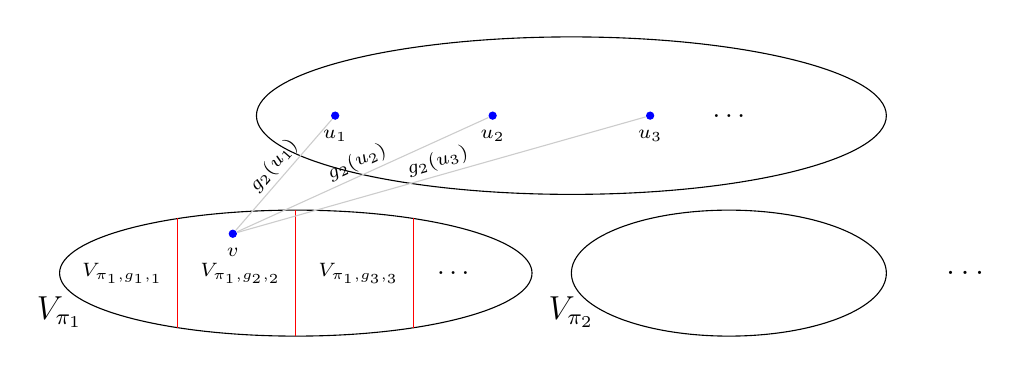
\begin{tikzpicture}
                \draw (0,0) ellipse (4cm and 1cm);
                \node at (-3, 1) {\large $\cH$}; 

                \node[circle,fill=blue,inner sep=0pt,minimum size=3pt,label=below:{\scriptsize $u_1$}] (v1) at (-3, 0) {};
                \node[circle,fill=blue,inner sep=0pt,minimum size=3pt,label=below:{\scriptsize $u_2$}] (v2) at (-1, 0) {};
                \node[circle,fill=blue,inner sep=0pt,minimum size=3pt,label=below:{\scriptsize $u_3$}] (v3) at ( 1, 0) {};
                \node at ( 2, 0) {$\ldots$}; 

                \draw (-3.5, -2) ellipse (3cm and 0.8cm);
                \node at (-6.5,-2.5) {\large $V_{\pi_1}$}; 

                \node at (-5.7,-2) {\scriptsize $V_{\pi_1, \tuple{g_1, \bff_1}}$};
                \node at (-4.2,-2) {\scriptsize $V_{\pi_1, \tuple{g_2, \bff_2}}$};
                \node at (-2.7,-2) {\scriptsize $V_{\pi_1, \tuple{g_3, \bff_3}}$};
                \node at (-1.5,-2) {$\ldots$}; 
                \draw[red] (-5,  -1.3) -- (-5,  -2.7);
                \draw[red] (-3.5,-1.2) -- (-3.5,-2.8);
                \draw[red] (-2,  -1.3) -- (-2,  -2.7);

                \node[circle,fill=blue,inner sep=0pt,minimum size=3pt,label=below:{\scriptsize $v$}] (u) at (-4.3, -1.5) {};

                \draw[gray!40] (v1) --  node[color=black,above=-2,sloped] {\scriptsize $g_2(u_1)$} (u);
                \draw[gray!40] (v2) --  node[color=black,above=-2,sloped] {\scriptsize $g_2(u_2)$} (u);
                \draw[gray!40] (v3) --  node[color=black,above=-2,sloped] {\scriptsize $g_2(u_3)$} (u);

                \draw (2, -2) ellipse (2cm and 0.8cm);
                \node at (0,-2.5) {\large $V_{\pi_2}$}; 

                \node at (5,-2) {\large $\ldots$}; 
            \end{tikzpicture}
        \end{center}
        \caption{An illustration of the model construction extending the partial model $\cH$  for the proof of Theorem~\ref{lem:c2_spec_core}.}
        \label{fig:construct}
    \end{figure}


    \textbf{\uline{Suppose that $\bfv \in \sol{\Psi^\varphi_\cH(\bfx)}$}}.
    For every $\pi \in \onetypes^\varphi$ and
    $\tuple{g, \bff} \in \cB^\varphi_{\pi, \cH}$,
    let $a_\pi$ be the $\pi^{th}$ component of $\bfv$ and
    $b_{\pi, \tuple{g, \bff}}$ be the corresponding assignment to $\bfy$.
    Our goal is to construct a finite model $\cG$ of $\varphi$ by extending the partial model $\cH$.
    The construction is illustrated in Figure~\ref{fig:construct}.
    We extend the partial model $\cH$ by introducing sets of fresh vertices $V_{\pi, \tuple{g, \bff}}$,
    where the cardinality of each set is $b_{\pi, \tuple{g, \bff}}$.
    All vertices in $V_{\pi, \tuple{g, \bff}}$ are assigned the 1-type $\pi$.
    Let $V_{\pi}$ be the union of $V_{\pi, \tuple{g, \bff}}$ for every $\tuple{g, \bff}$.

    We handle edge coloring using a four-step procedure which we now outline.
    Firstly, we
    color edges between the core $\cH$ and the relative complement of the core $\cG \setminus \cH$.
    In steps two and three,
    we iterate over all pairs of 1-types $\pi_1$ and $\pi_2$ realized in the relative complement of the core $\cG \setminus \cH$ and color edges between $V_{\pi_1}$ and $V_{\pi_2}$ as follows:
    \begin{itemize}
        \item In step 2, we color edges with 2-types that are neither forward-silent nor backward-silent.
        \item In step 3, we color edges with 2-types that are not forward-silent,  but which are backward-silent.
    \end{itemize}
    We mention that the following invariant will be maintained during the iteration described above:

    \medskip

    For every $\pi \in \onetypes^\varphi$ and $\tuple{g, \bff} \in \cB^\varphi_{\pi, \cH}$,
    for every vertex $v$ in $V_{\pi, \tuple{g, \bff}}$,
    for every $\pi' \in \onetypes^\varphi$ and $\eta \in \cKvpf_{\pi, \pi'} \cup \cKvpfb_{\pi, \pi'}$,
    the number of colored edges from $v$ to $V_{\pi'}$ with 2-type $\eta$ is either 0 or $\bff(\eta, \pi')$.

    \medskip

    After the iteration, in step 4 we handle the remaining edges with 2-types that are both forward- and backward-silent.
    
    We now provide the details of the procedure.
    \begin{enumerate}
        \item 
            For every $v$ in $\cG \setminus \cH$  and $u$ in $\cH$,
            we add an edge between $v$ and $u$ with 2-type $g(u)$.
        \item
            For every $\pi_1, \pi_2 \in \onetypes^\varphi$,
            we assign audible 2-types in $\cKvpfb_{\pi_1, \pi_2}$ and $\cKvpfb_{\pi_2, \pi_1}$
            between $V_{\pi_1}$ and $V_{\pi_2}$.
            We first assume that parallel edges are allowed,
            Because $b_{\pi, \tuple{g, \bff}}$ is a solution of $\match_{1, \cH}(\bfy)$,
            it is straightforward to assign (parallel) edges between $V_{\pi_1}$ and $V_{\pi_2}$ 
            such that
            \begin{itemize}
            \item
                for every $v \in V_{\pi_1, \tuple{g, \bff}}$, for every $\eta \in \cKvpfb_{\pi_1, \pi_2}$,
                the number of edges from $v$ to $V_{\pi_2}$ with 2-type $\eta$ is exactly $\bff(\eta, \pi_2)$.
            \item
                for every $v \in V_{\pi_2, \tuple{g, \bff}}$, for every $\eta \in \cKvpfb_{\pi_2, \pi_1}$,
                the number of edges from $v$ to $V_{\pi_1}$ with 2-type $\eta$ is exactly $\bff(\eta, \pi_1)$.
            \end{itemize}

            To eliminate parallel edges in the above construction,
            we again apply a swapping procedure, as in \cite{tonyeryk,ultimatelyperiodic}.
            Note that each vertex $v \in V_{\pi_1} \cup V_{\pi_2}$ is adjacent to at most $K^\varphi$ edges.
            Suppose that there are parallel edges $e_1$ and $e_2$
            between $v_1 \in V_{\pi_1}$ and $v_2 \in V_{\pi_2}$ with the 2-type of $e_1$ being $\eta_1$ and
            the $2$-type of $e_2$ being $\eta_2$.
            Let $u_1 \in V_{\pi_1}$ and $u_2 \in V_{\pi_2}$ be vertices such that
            there is an edge $e_3$ between them with 2-type $\eta_2$,
            $u_1$ is not adjacent to $v_2$, and
            $u_2$ is not adjacent to $v_1$.
            Because $b_{\pi, \tuple{g, \bff}}$ is a solution of $\bige_{\cH}(\bfy)$,
            there are at least $(2K^\varphi+1)^2$ edges from $V_{\pi_1}$ to $V_{\pi_2}$ with 2-type $\eta_2$.
            Since each of $v_1$ and $v_2$ has at most $K^\varphi$ adjacent edges,
            it is always possible to find such $u_1$ and $u_2$.
            We then remove the edges $e_2$ and $e_3$,
            and replace them with fresh edges $(v_1, u_2)$ and $(v_2, u_1)$ with 2-type $\eta_2$.
            This swapping procedure preserves the number of edges connected to vertices with specific 2-types
            but reduces the number of parallel edges by 1,
            We can repeat this until all parallel edges are eliminated.

        \item
            For every $\pi_1, \pi_2 \in \onetypes^\varphi$,
            we assign backward-silent but not forward-silent 2-types in $\cKvpf_{\pi_1, \pi_2}$ and $\cKvpf_{\pi_2, \pi_1}$
            between $V_{\pi_1}$ and $V_{\pi_2}$.
            Again, we assume first that parallel edges are allowed,
            Because $b_{\pi, \tuple{g, \bff}}$ is a solution of $\match_{2, \cH}(\bfy)$,
            if $\sum_{\tuple{g, \bff} \in \cB^\varphi_{\pi_1, \cH}} \bff(\eta, \pi_2) \cdot b_{\pi_1, \tuple{g, \bff}} > 0$,
            then $\sum_{\tuple{g, \bff} \in \cB^\varphi_{\pi_2, \cH}} b_{\pi_2, \tuple{g, \bff}} > 0$,
            which implies that $V_{\pi_2}$ is not empty.
            Thus we can assign (parallel) edges from $V_{\pi_1}$ and $V_{\pi_2}$ satisfying that
            \begin{itemize}
            \item
                for every $v \in V_{\pi_1, \tuple{g, \bff}}$, for every $\eta \in \cKvpf_{\pi_1, \pi_2}$,
                the number of edges from $v$ to $V_{\pi_2}$ with 2-type $\eta$ is exactly $\bff(\eta, \pi_2)$.
            \end{itemize}
            A similar argument applies to edges from $V_{\pi_2}$ to $V_{\pi_1}$.
            \begin{itemize}
            \item
                for every $v \in V_{\pi_2, \tuple{g, \bff}}$, for every $\eta \in \cKvpf_{\pi_2, \pi_1}$,
                the number of edges from $v$ to $V_{\pi_1}$ with 2-type $\eta$ is exactly $\bff(\eta, \pi_1)$.
            \end{itemize}

            We apply the swapping procedure to eliminate parallel edges as well.
            Suppose that there are parallel edges $e_1$ and $e_2$
            between $v_1 \in V_{\pi_1}$ and $v_2 \in V_{\pi_2}$ with 2-types $\eta_1 \in \cKvpf_{\pi_1, \pi_2}$ for $e_1$ and $\eta_2$ for $e_2$.
            We consider two cases:
            \begin{itemize}
            \item 
                If there is a vertex $u_2 \in V_{\pi_2}$ such that there is no edges between $v_1$ and $u_2$,
                then we remove $e_1$ and add an edge between $v_1$ and $u_2$ with 2-types $\eta_1$.
            \item 
                Otherwise, suppose that there is no such $u_2$,
                which implies that for every vertex $u \in V_{\pi_2}$,
                there exists an edge $e_3$ between $v_1$ and $u$.
                Because there are at most $2K^\varphi(2K^\varphi+1)^2$ edges
                between $V_{\pi_1}$ and $V_{\pi_2}$,
                we can find $u_1 \in V_{\pi_1}$ and $u_2 \in V_{\pi_2}$
                such that no edges exists between them,
                and there exists an edge $e_3$ between $v_1$ and $u_2$ with type $\eta_3 \in \cKvpb_{\pi_1, \pi_2}$. 
                We then remove the edges $e_1$ and $e_3$
                and fresh edges $(v_1, u_2)$ with 2-type $\eta_1$ and $(v_2, u_2)$ with 2-type $\eta_3$.
            \end{itemize}
            For both cases, the swapping procedure preserves the number of edges connected to vertices with specific 2-types
            but reduces the number of parallel edges by 1,
            We can repeat it until all parallel edges are eliminated.

        \item
            Finally, for every pair of vertices $v_1 \in V_{\pi_1}$ and $v_2 \in V_{\pi_2}$ 
            with no edge connected,
            we add an edge between them with a 2-type  $\eta \in \cKvpnull_{\pi_1, \pi_2}$.
    \end{enumerate}

    We first claim that the 1-type cardinality vector of $\cG$ is exactly $\bfv$.
    For every $\pi \in \onetypes^\varphi$,
    recall that the number of vertices in $\cH$ with 1-type $\pi$ is $s_\pi$.
    The number of vertices in $\cG \setminus \cH$ with 1-type $\pi$ is
    $\abs{V_\pi} = \sum_{\tuple{g, \bff} \in \cB^\varphi_{\pi, \cH}} \abs{V_{\pi, \tuple{g, \bff}}} = \sum_{\tuple{g, \bff} \in \cB^\varphi_{\pi, \cH}} b_{\pi, \tuple{g, \bff}}$.
    Since $a_\pi$ and $b_{\pi, \tuple{g, \bff}}$ is a solution of $\summ_{\cH}(\bfx, \bfy)$,
    we have $a_\pi = s_\pi + \sum_{f \in \cB^\varphi_{\pi, \cH}} b_{\pi, \tuple{g, \bff}}$.
    Recall that $a_\pi$ is the $i^{th}$ component of $\bfv$, where $i$ is the index of $\pi$ in the  ordering of $\onetypes^\varphi$.
    Thus the 1-type cardinality vector of $\cG$ is exactly $\bfv$.

    We next claim that $\cG$ is a model of $\varphi$, by checking the conditions in Proposition~\ref{prop:ctwo_graph}.
    It is routine to check that all vertices and edges in $\cG$ satisfy the 1- and 2-type conditions.
    Thus it is sufficient to check that the counting condition holds for every vertex $v$ in $\cG$.
    \begin{itemize}
        \item
        For every $v$ in $\cH$, note that
        \begin{equation*}
            \sum_{u \in V_{\pi, \tuple{g, \bff}}} \twotypeof^\trif(v, u) 
            \ =\ 
            \sum_{u \in V_{\pi, \tuple{g, \bff}}} g^\trib(v)
            \ =\ 
            g^\trib(v) \cdot \abs{V_{\pi, \tuple{g, \bff}}}
            \ =\ 
            g^\trib(v) \cdot b_{\pi, \tuple{g, \bff}}.
        \end{equation*}
        Because $b_{\pi, \tuple{g, \bff}}$ is a solution of $\comp_{\cH}(\bfy)$, we have
        \begin{equation*}
            \begin{aligned}
                \sum_{u \in V \setminus \set{v}} \twotypeof^\trif(v, u)
                \ =\ &
                \sum_{u \in V_c \setminus \set{v}} \twotypeof^\trif(v, u) +
                \sum_{\pi \in \onetypes^\varphi}\sum_{\tuple{g, \bff} \in \cB^\varphi_{\pi, \cH}}\sum_{u \in V_{\pi, \tuple{g, \bff}}} \twotypeof^\trif(v, u) \\
                \ =\ &
                \sum_{u \in V_c \setminus \set{v}} \twotypeof^\trif(v, u) +
                \sum_{\pi \in \onetypes^\varphi}\sum_{\tuple{g, \bff} \in \cB^\varphi_{\pi, \cH}} g^\trib(v)\cdot b_{\pi, \tuple{g, \bff}} \\
                \ =\ &
                \bfk^\varphi
            \end{aligned}
        \end{equation*}

        \item
        For every $v \in V_{\pi, \tuple{g, \bff}}$,
        note that the extended behavior of $v$ is $\tuple{g, \bff}$.
        Since $\tuple{g, \bff} \in \cB^\varphi_{\pi, \cH}$,
        by the compatibility condition in Definition~\ref{def:compatextended}, it holds that
        \begin{equation*}
            \begin{aligned}
                \sum_{u \in V \setminus \set{v}} \twotypeof^\trif(v, u)
                \ =\ &
                \sum_{u \in V_c} \twotypeof^\trif(v, u) +
                \sum_{u \in V \setminus (V_c \cup \set{v})} \twotypeof^\trif(v, u) \\
                \ =\ &
                \sum_{u \in V_c} g^\trif(u) + 
                \sum_{\pi' \in \onetypes^\varphi}
                \left(
                    \sum_{\eta \in \cKvpf_{\pi, \pi'}} \bff(\eta, \pi') \cdot \eta^\trif +
                    \sum_{\eta \in \cKvpfb_{\pi, \pi'}} \bff(\eta, \pi') \cdot \eta^\trif
                \right) \\
                \ =\ &\bfk^\varphi
            \end{aligned}
        \end{equation*}
    \end{itemize}
\end{proof}
